\documentclass[]{algotel}
\usepackage[utf8]{inputenc}
\usepackage[english]{babel}

\usepackage{xspace}
\usepackage{graphicx,graphics} 
\usepackage{hyperref} 
\usepackage{mathtools, bm}
\usepackage{amssymb, bm}
\usepackage{complexity}
\usepackage{amsthm}
%\usepackage{authblk}
\usepackage{color}
\usepackage{amsmath}


\newcommand\pall{\textsc{pall}\xspace}


\newcommand{\todo}[1]{{\color{red} TODO: {#1}}}	
\newtheorem{prop}{Proposition}


\graphicspath{{img/}}

%opening
\title{Contention management for Cloud Ran over an optical ring}

%\author[1]{Dominique Barth}
%\author[2]{Dominique Chiaroni ?}
%\author[1]{Ma\"el Guiraud}
%\author[1]{Yann Strozecki}
%\affil[1]{David Laboratory, UVSQ}
%\affil[2]{Nokia Bell Labs France}




\author{Dominique Barth\addressmark{1}
  \and Dominique Chiaroni?\addressmark{2}
  \and Ma\"el Guiraud \addressmark{1,2}
   \and Yann Strozecki \addressmark{1}
  }

\address{\addressmark{1}David Laboratory, UVSQ \\
  \addressmark{2}BNokia Bell Labs France}
\keywords{N-GREEN, Optical ring, Latency, 5G}

\begin{document}

\maketitle


\begin{abstract}

% Nowadays challenge for network providers is to design some network which satisfies in the same time a good Quality of Services and a cheap hardware development.
This study is a contribution to the N-GREEN project, which has for goal to design a low cost optical ring technology with good performances (dataflow, latency,$\dots$) without using expensive end to end connections. In this paper, we study the compatibility of such a technology with the development of the Cloud Ran, a latency critical application which is a major aspect of the 5G deployment. We show that the latency of the Cloud Rand can be guaranteed by using a deterministic sending scheme without impacting the others traffics. 
\end{abstract}

\todo{ça marque et dans le titre, ça ne devrait pas

Il faut citer l'ANR NGREEN + n'importe quel truc de charoni qui explique leur architecture NGREEN}


\section{Introduction}

Network providers have to design inexpensive networks while the amount of data and online applications significantly increases. Much of these applications have QoS criteria, like a minimal bandwidth or a maximal latency. The N-GREEN project aims to propose an high performing optical ring while ensuring a minimal cost for providers. The current solutions with good QoS [huawei, demander a dominique C], establishes end to end connection (E2E) between the nodes, which is extremely expensive. The N-GREEN optical ring is designed to ensure good performances and the hardware it requires scales linearly with the number of nodes while E2E scales quadratically making it impractical for more than a few nodes.

In this article, we study a Cloud RAN application in the N-GREEN optical ring. Cloud RAN is one of the major area of development for 5G, that consists in centralizing the computation units (or {\bf BaseBand Units, BBU}) of the Remote Radio Heads ({\bf RRHs}) in one {\bf datacenter}. The latency of the messages between the BBU and the RRH is critical \cite{}. Here, we study the latency of some C-RAN equipment connected through an N-GREEN optical ring.\todo{mettre les citations, à reprendre de nos précédents articles}

\todo{Dire un mot sur la forme du traffic cloud RAN, périodique déterministe, aller vers un data center unique, retour, minimisation de la latence ...}

In Sec.~\ref{sec:model}, we model the optical ring and the traffic flow we study. In Sec.~\ref{sec:oportmethods}, we study the latency when using stochastic multiplexing to manage the messages arrivals on the ring, with or without priority of the C-RAN traffic. Finally, in Sec.~\ref{sec:deterministicalgorithms}, we propose deterministic ways to manage the C-RAN without buffers and thus with a minimal latency compared to stochastic multiplexing. The best method also improve the latency of the rest of the traffic.
\todo{Je sais pas si il faut parler de SDN, qui est un keyword a la mode mais peut etre que l'architecture ngreen nous propose, demander a chiaroni, 
Yann : je pense qu'il faut parler de SDN, reprendre peut être des choses de notre article précédent sur Cloud RAN}


\section{Model of C-RAN traffic over an optical ring}
\label{sec:model}
% 
%   \subsection{Network modeling}
% 
% The model exposed here has already been studied for another particular topology of network and with different problematics from the ones of this paper. One can find in \cite{latency2017} the complexity results on the problem proposed, and some algorithmic solutions to solve it in star networks.
          
  \subsection{N-GREEN Optical ring}
   
  The unidirectional optical ring is represented by an oriented cycle. The vertices of the cycle represents the nodes of the ring, where traffic arrives. The edges $(u,v)$ of the cycle have an integer weight $\omega(u,v)$ which represents the time to transmit a unit of information from $u$ to $v$. We denote by $RS$ (ringsize) the length of the cycle, that is the sum of $\omega(u,v)$ for all arcs $(u,v)$.  Each arc $(u,v)$ can be seen as a sequence of $\omega(u,v)$ {\bf containers}, of capacity $Z$, expressed in Bytes.  The containers are filled  by the nodes with smaller packets called {\bf Packet Data Unit}, or PDU.
  PDUs waiting in the node $u$ can be put in the first container of the arc $(u,v)$ \emph{if it is free}. 
  The dynamic of the network is simple: at each unit of time PDUs contained in a container go to the next.
   The ring follows a {\bf broadcast and select with emission release policy}. When a container is filled by some node $u$,
   it is freed when it comes back at $u$ after a whole round trip.
   
   \subsection{C-RAN trafic}
   
   We study a C-RAN traffic emitted by each RRH. The data from an antenna arrives into a specific node, then it is routed to 
   its BBU through the ring. Then after some computation time (which is here supposed to be zero to simplify the model),
   an answer is sent back from the BBU to the RRH. The same quantity of data is emitted by an antenna at each period $P$. 
   In our model all BBUs are in the same data-center, thus they are all attached to the same node of the ring. In the following, we will denote by $n$ the number of antennas.
   
   The antenna are linked to the nodes of the ring through an electronic interface of rate $D$Bps.
   The ring has a larger rate of $KD$Bps. The integer $K$ is called the {\bf acceleration factor} between the electronic and the optical domains. A node aggregates the data received on the electronic interface during $K$ unit of times to create a PDU of size $Z$, that is which can fills one container of the ring. As a consequence, we consider that each period, an antenna emits a PDU of size $Z$ each $K$ unit of times during a time $ET$.
    
\begin{figure}[h!]
\begin{center}   

      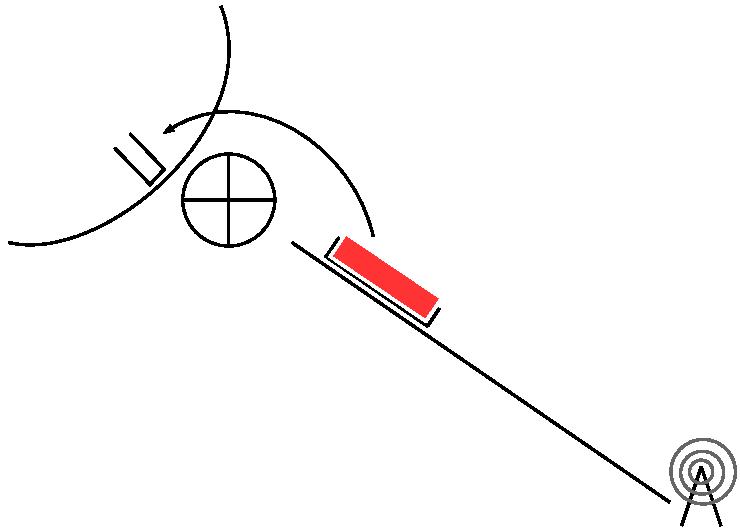
\includegraphics[scale=0.2]{slot1.pdf}
  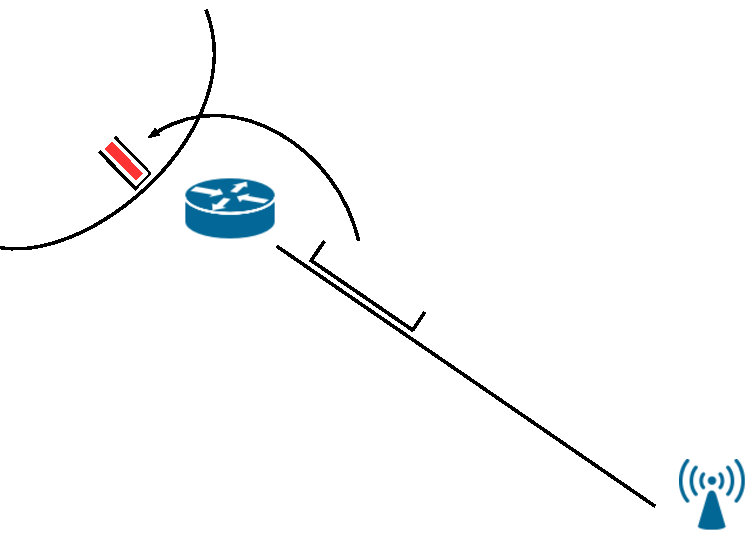
\includegraphics[scale=0.2]{slot2.pdf}
     \caption{Opto-electronic interface.}
     
\end{center}
  \end{figure}
  \todo{Améliorer le dessin: un seul schéma avec les notations et horizontal pour pas perdre de place.
  Éventuellement faire une représentation du ring et en zoom faire l'interface}
%   
%       An node deals with two kinds of traffics. Some C-RAN and some Best Effort. We assume that each traffic has its corresponding electronic interface. Also, a C-RAN message is of size $Z$ and completely fills a container let us call {\bf C-RAN PDU} such a message. In the same time, the Best Effort messages are buffered in a first {\em gathering buffer} before being gathered together into a {\bf BE PDU}. Once the PDUs are created, there join the {\em contention buffer} before being sent in the ring.  
%       \begin{figure}[h!]
% \begin{center}   
%   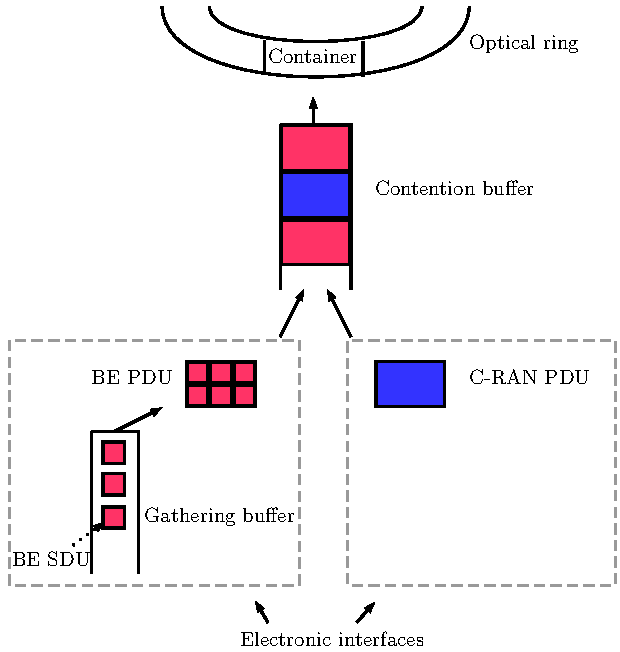
\includegraphics[scale=0.7]{buffers.pdf}
%      \caption{An N-GREEN station.}
%      
% \end{center}
%   \end{figure}
%  
   
%    
%   The C-RAN PDUs coming from an antenna are sent according to a 
%   
%   follows 
%   This study focuses on the performances of the C-RAN PDUs, thus the route we consider are the routes between the BBUs and the RRHs .We assume that there is a bijection between the RRHs and the BBUs.
%  We call forward routes the routes going from the RRHs to the BBUs and Backward routes the routes going from the BBUs to the RRHs. The addition of the weight of the two routes of a couple BBU-RRH is then equal to $RS$, the size of the ring, measured in slots. We denote by $n$ the number of couples BBU-RRH.
%  We only consider one data center into the ring. This mean that all the forward routes have the same destination nodes, and all the backward routes have the same source node.

% 
% 
% \subsection{Into the node : Two kind of traffics}

\todo{Décrire ici les degrés de liberté -> quand ça part + la latence}


\subsection{Best effort traffic}

\todo{Décrire la génération du best effort}

\paragraph{BE PDU generation model} To Generate the BE PDU, we used the distribution of the time between the generation of two BE PDU given by some numerical analysis work of another study for N-GREEN. This distribution was calculated by modeling a gathering buffer.
  
 \paragraph{C-RAN PDU generation model} An RRH usually emit an huge quantity of information during a long time. Also, as we just see, an RRH can send no more than a PDU every $K$ slots on the ring.
 We denote by $ET$,for {\bf Emission time}, the time during which an RRH emits a PDU every $K$ slots on the ring. An RRH emits $\frac{ET}{K}$ PDUs on the ring, every period $P$.
    	    
        \begin{figure}[h!]
\begin{center}   

      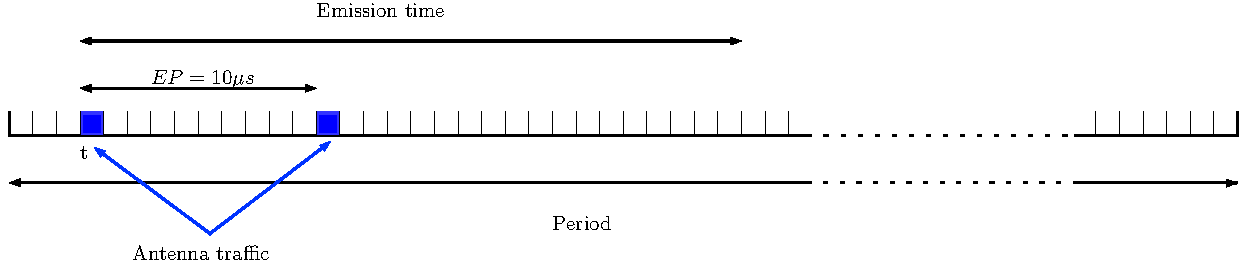
\includegraphics[width=\textwidth]{emission_antenna.pdf}
     \caption{C-RAN PDU generation.}
\end{center}
  \end{figure}
  \paragraph{Back and forth communications} As we explained in the introduction of this section, once the datacenter receives some PDUs from an RRH, it computes an answer and send it to the RRH through the ring. To simplify our model, we assume that the computation times is the same for all BBUs and that it is a multiple of the period. In this situation, we can assume that, each time the datacenter receives a container with a C-RAN PDU from an RRH, it immediately sends an answer (which is in fact the answer to the two periods ago C-RAN PDU's).
  
  The time at which an RRH on the route $r_i$ sends its first PDU is called {\bf offset} and can be expressed by $m_{r_i}$. The time at which this first PDU arrives to its BBU is the {\bf BBU-offset}, $t(v,r_i) = m_{r_i} + \omega(u,v)$, where $u$ is the RRH and $v$ the BBU of the route $r_i$.
  We denote by {\bf latency} of a PDU the time sojourn time of a PDU in the contention buffer.
  We want to ensure a good latency for the C-RAN PDUs. If there is no BE PDUs on the ring, the challenge is to fix the offsets (that directly fixes the BBU-offsets) of the routes such that two messages never collides each others. Nevertheless, we have ton consider the BE PDUs in our model.
 The rest of this study is divided in two parts. In a first time, we look at the behaviour of the ring and the impact of the PDUs latency with two different method of managing the contention buffer. Then, we propose some algorithms that solve allows us to choose the offsets for the C-RAN PDUs by reserving the containers, and we compare the impact of those different algorithms on the BE PDUs latency.

  \subsection{Parameters of the study}
  \label{sec:parameters} The experiment of this subsections are made following the same parameters, until sec~\ref{sec:optialgo}. We set $K = 10$ chanels, some electronic interface of rate $D=10$Gbps and $Z = 12500$B so, $Z/KD = 1\mu$s. The optical ring has a rate $KD=100$Gbps, while a slots has a duration of $1\mu$s. The length of the ring is to $20$km in our simulations, this means that the ring has a length of $RS = 100$ slots. We consider some BE SDUs of $125$B, and we parametrized BE PDU generator of sec~\ref{jmf} such that each node load the network with an average of $3,5\%$ of BE traffic. We set $ET = 500$ slots, that correspond to a C-RAN traffic of $5$Gbps. The period  $P$ is to $1$ms, that is $1000$ slots. We set the number of RRH to $n=5$. We take $5$ nodes and one of them is the datacenter. The antennas are apportioned between the others node. With those parameters, the network is theoretically loaded to $67.5\%$. 
  
  \begin{figure}
  \centering
  \begin{tabular}{|c|c|}
  \hline
 Number of channels $K$ & $10$  \tabularnewline
  \hline
  Rate of an electronic interface $D$ & $10$ Gbps \tabularnewline
  \hline
  Container size  $Z$ & $12,500$ B  \tabularnewline
  \hline
  Slot duration $Z/KD$ & $1\mu$s \tabularnewline
  \hline
  Optical ring rate $KD$ & $100$ Gbps \tabularnewline
  \hline
  Length of the ring $RS$ & $100$ slots \tabularnewline
  \hline
  BE SDU size & $125$B \tabularnewline
  \hline
  C-RAN PDU size & $12,500$B$=Z$ \tabularnewline
  \hline
  Emission time $ET$ & $500$ slots \tabularnewline
  \hline
   Period $P$ & $1,000$ slots \tabularnewline
  \hline
  Number of RRH & $5$  \tabularnewline
  \hline
  Number of nodes $n$ & $5$  \tabularnewline
  \hline
  
  \end{tabular}
  \caption{Parameters of the following experiments based on N-GREEN}\label{parameters}
  \end{figure}
  
   \section{Performance evaluation of the N-GREEN optical ring}
   \label{sec:oportmethods}
   In a first time, we will look at the performance of the N-GREEN optical ring with an opportunistic insertion policy. When a node wants to send a PDU on the ring, it uses the first available container .
    We study the performance of the ring through two methods; a full opportunistic method, and a method that prioritize the C-RAN PDUs. Since we only consider some PDUs arrivals, those two methods are some variants of the management of the PDUs in the node.
   For those two methods, the offsets $m_r$ of the routes are chosen randomly in the period, i.e. we do not choose the first time at which the RRH start to emit.

    
    \subsection{Full opportunistic method}
    \label{sec:fullopport}
    We first want to look at a simple configuration in which we do not manage the PUDs (BE or C-RAN) arriving into a node. At their arrival, the BE and C-RAN PDUS are buffered in the contention buffer, and this buffer is emptied following the FIFO rule.

The following experiment shows us the performance this {\bf full opportunistic method} with some parameters issued from N-GREEN. 
On fig~\ref{fig:oport}, one can see the cumulative distribution of the latency of the C-RAN and BE PDUs. Those results are computed on $100$ instances of optical rings that have run during $10,000,000$ slots. The measures are taken after $3,000$ slots of simulation, to let the ring initialize it's behavior. The parameters of the simulations are stated in sec~\ref{sec:parameters}.


    \begin{figure}[h!]
    \label{fig:oport}
        \begin{center}
      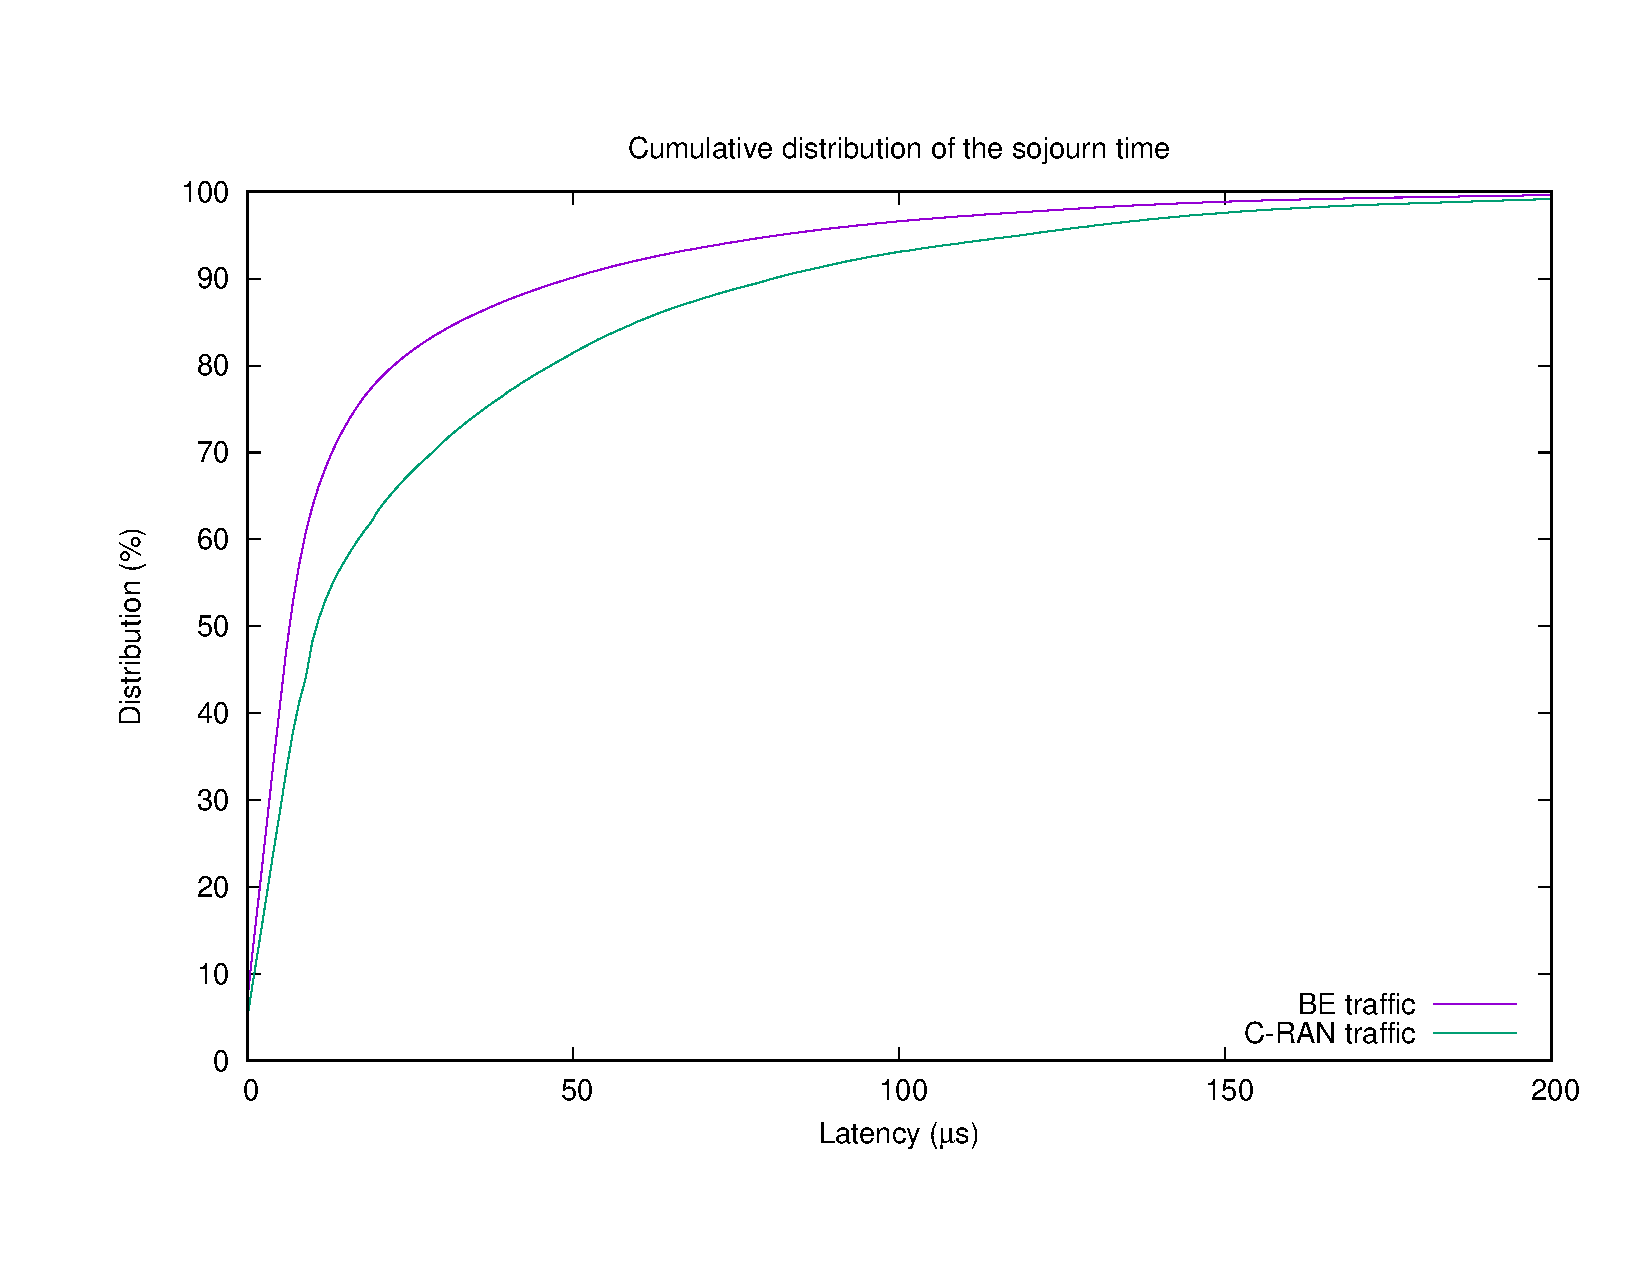
\includegraphics[scale=0.4]{oport}

      \caption{Full opportunistic method performances.}
      \end{center}
  \end{figure}
  
  As we can see on fig~\ref{fig:oport}, the latency for the different kind of PDU is notably similar because we do not manage anything. Furthermore, we can remark that about $10\%$ of the C-RAN messages wait over $100\mu$s, that is already critical for C-RAN \todo{ref}.

\subsection{C-RAN priority method}
\label{sec:cranprio}
  In order to improve the C-RAN PDUs latency, we imagined the following solution, called {\bf C-RAN priority method}. Each nodes have two contention buffers. One for the BE PDUs, and one fore the C-RAN PDUs. When a node is able to send a PDU on the ring, i.e. its available container is free, the container is filled with the C-RAN PDUs first. 
  
    \begin{figure}[h]
\begin{center}   
      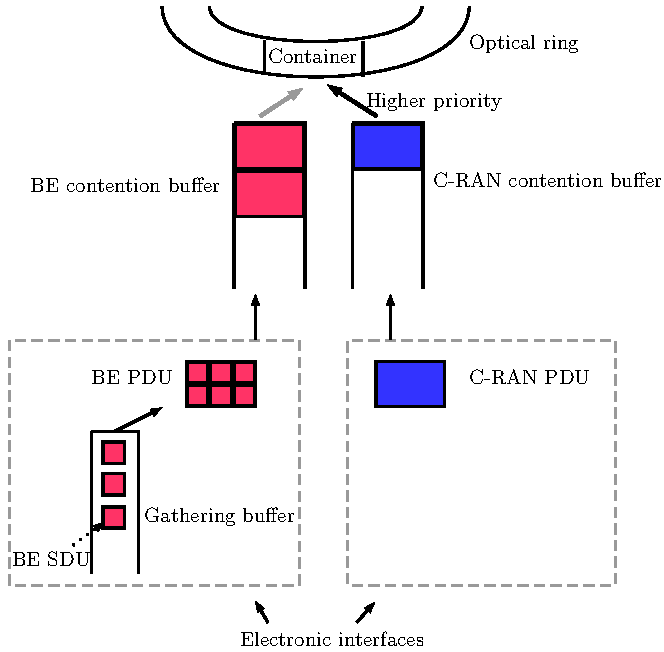
\includegraphics[scale=0.7]{cranprio.pdf}
     \caption{C-RAN priority method.}
\end{center}
  \end{figure}
  
  With this method, one can imagine improve the latency of the C-RAN PDUs. Fig~\ref{fig:prior} shows us the performance of the C-RAN priority algorithm for different kinds of traffics. The parameters of the simulations still the same, stated in sec~\ref{sec:parameters}.
      \begin{figure}[h]
      \label{fig:prior}
\begin{center}   

      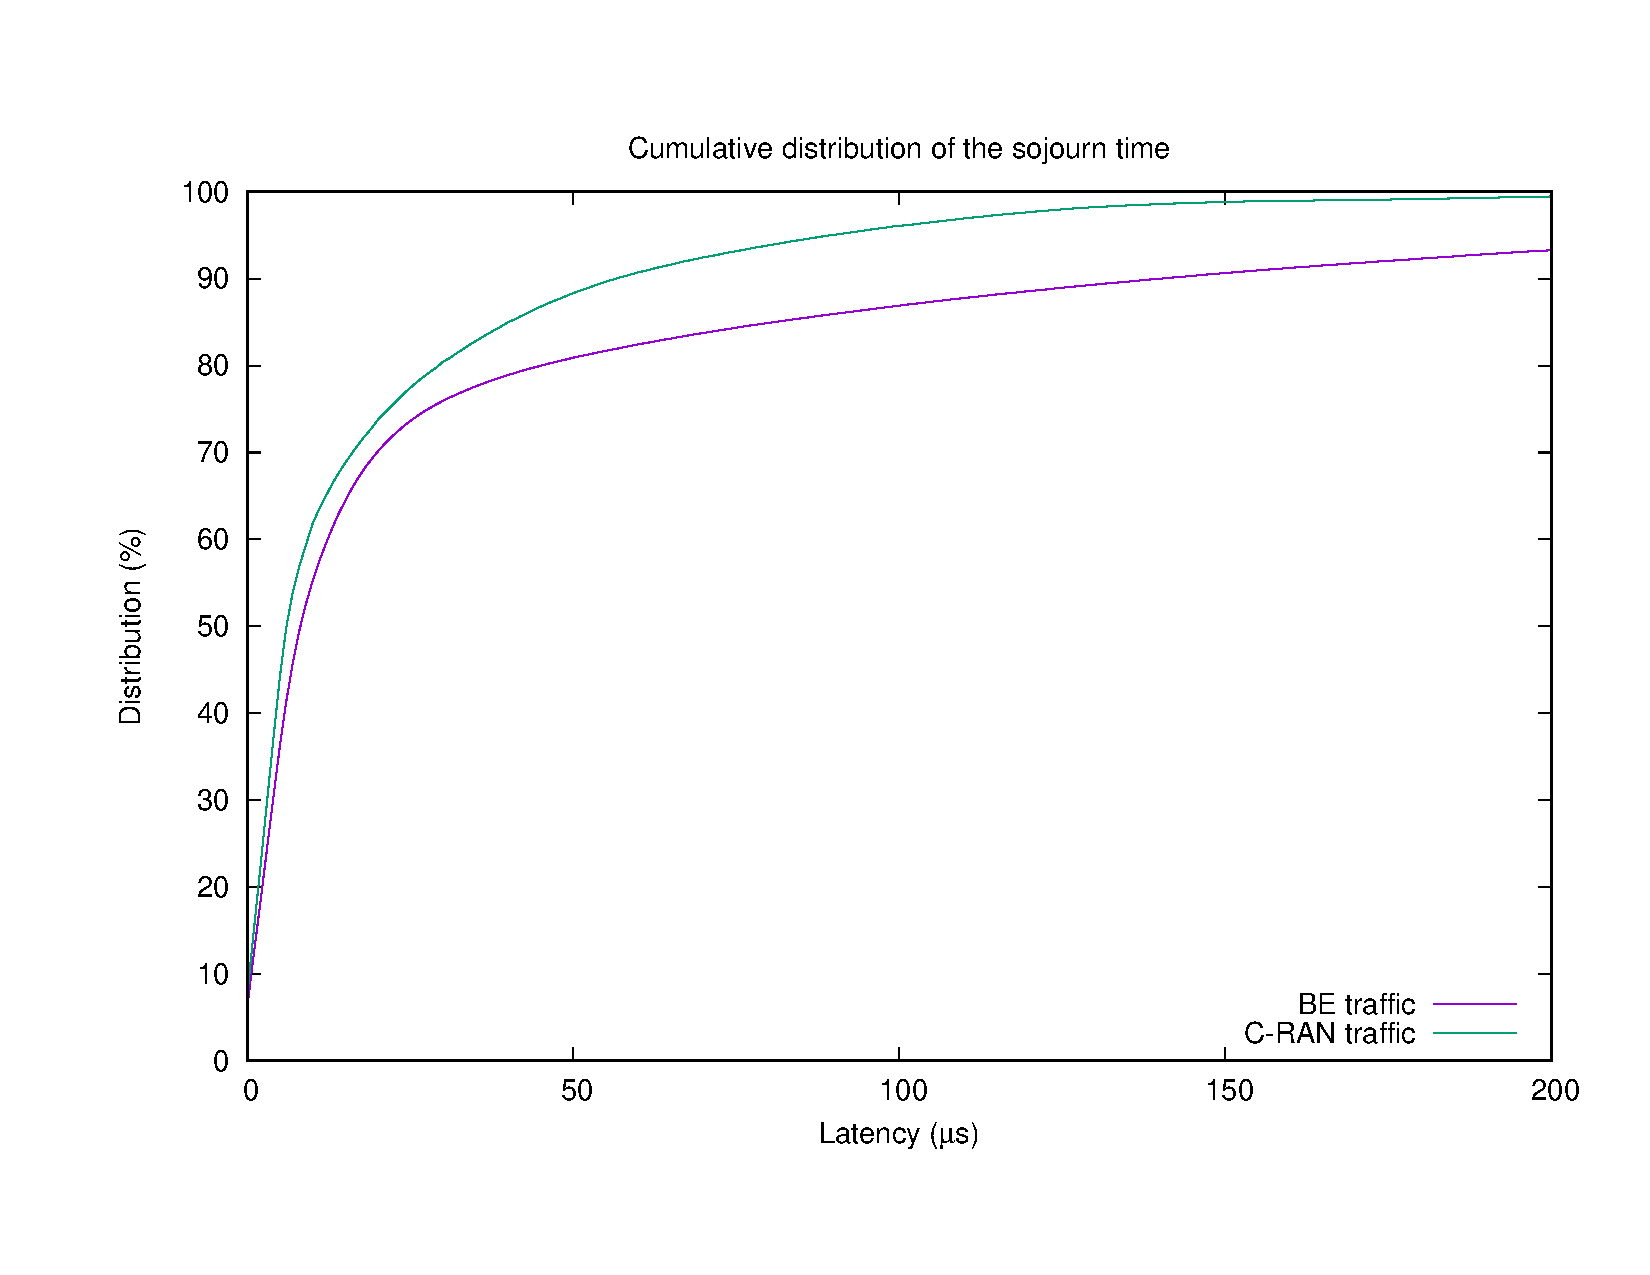
\includegraphics[scale=0.4]{prior.pdf}

     \caption{C-RAN priority method performances.}
\end{center}
  \end{figure}
  
  As expected, the latency of the C-RAN PDUs is decreased compared to the full opportunistic method. Nevertheless, there is still $10\%$ of the C-RAN PDUs that have more than $50 \mu$s of latency, and the best effort PDUs are penalized, indeed, close to $10\%$ of the BE PDUs awaits more than $150\mu$s before being sent in the ring, versus close to $0\%$ with the previous method..
  Thus, we propose a deterministic approach in which we set the offsets of the RRH and we reserve the containers needed for the C-RAN PDUs.
   \todo{il manque une partie sur le travail de karim, }
  \section{Deterministic approach for $0$ latency on C-RAN}
\label{sec:deterministicalgorithms}

 In this section We present three algorithms that allows the C-RAN PDUs to have $0$ latency in the insertion buffers by establishing a static reservation of the slots in the period.
 Those algorithm are {\bf Centralized} and requires a global supervisor of the network to be implemented .\todo{phrase + ref sdn?}
 
\paragraph{Slot reservation} To decrease the C-RAN messages latency, one plan to reserve the container for the nodes. Indeed, if a node $i$ needs to send a PDU at time $t$, a container needs to be reserved since the previous lap of the container, i.e. at time $t - RS$ by $i$. In this situation, if the container is already taken by a PDU which has been sent by a node $j$, $j$ will remove the PDU of the container during the next lap of the ring, and no other nodes are able to write in this container before it comes back to the node $i$ a date $t$. By choosing the offsets of the route and reserving the corresponding containers, we allow the C-RAN PDUs to have $0$ latency in the nodes. Though, it impacts the best effort PDUs, by avoiding them to use free reserved containers. It is equivalent to increase the load of the network, without increasing the number of PDUs carried by the network. 

\paragraph{RRHs synchronisations}
This slot reservation implies that the RRHs are synchronized with the ring. The following proposed algorithms set a sequence of reserved slots for each RRH in each period. A technical application implies to simultaneously ensure the reservation of the slot to the given dates, and the synchronization of the RRH with those reserved slot. One must ensure that the C-RAN PDU arrives in the contention buffer of the node just before the reserved container.

  
Unlike the previous methods with opportunistic insertion policy, we now want to choose a the offsets for the routes. Since all the forward routes have the same last vertex $v$ (the datacenter), which is also the first vertex of all the backward routes, we choose to manage the collision in this vertex only. The purpose is then to determine the time BBU offset of the routes. Once the BBU-offsets are set, for all routes $i$, it is easy to compute $m_{r_i} = t(v,r_i) - \omega(u,v)$.


\subsection{N-GREEN parameters adapted algorithms}
An RRH can not emit a message more often than once slot every $K$ slots. Remember that {\bf macro slot} is a duration of $K$ slots, during which each RRH can emit at most once. Thus, we consider the simple case in which there is less C-RAN traffic than slots in a macro slot. Indeed, in that case, we only manage the collision in one macro slot, i.e. we assign a C-RAN traffic to each slot of the macro-slot. Since a BBU always instantly emits an answer to it's RRH, for each RRH, a group of two following containers (called {\bf bunch}) can be reserved. Thus, we first study the case $K \ge 2\times n$. As a reminder, $n$ is the number of couple BBU-RRH. 

 
 Because there is at most as much couples BBU-RRH as bunches, we want to assign one RRH to one bunch.
We propose the following {\bf naive reservation algorithm}. For each RRH $i, i\in \{0,...,n-1\} $, set $t(v,r_i)= 2\times i$ with $v$ the vertex of the BBUs. The model automatically fixes the offset of the backward route $\rho(r_i)$ to $m_{\rho(r_i)}= 2\times i +1$. This is the reason why we do not care about the backward routes anymore, and we only deal with the BBU-offsets of the forward routes..
   \begin{figure}[h]
\centering
      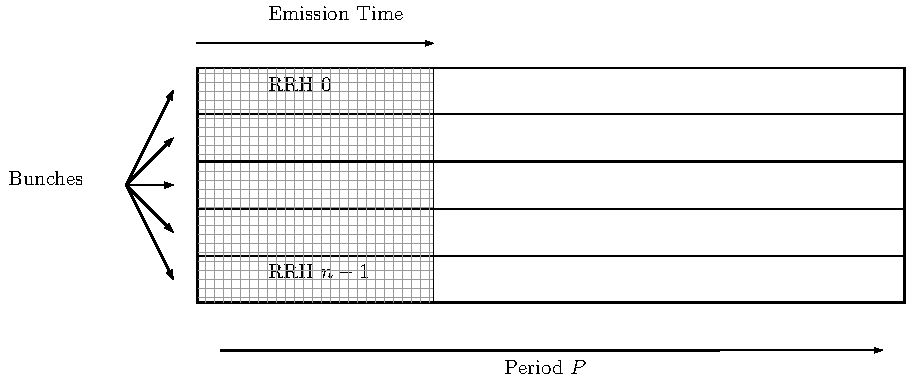
\includegraphics[scale=0.7]{freqgrouped.pdf}
     \caption{Grouped assignment of the bunches to the RRH.}   \label{fig:freqG}
  \end{figure}


We kept the same parameters than in the two previous experiments (see~\ref{sec:parameters}) and we made an experiment to show the impact of this algorithm on the BE traffic. Fig~\ref{fig:res1} shows us the distribution of latency for BE PDUs with this algorithm.

      \begin{figure}[h]
\centering
      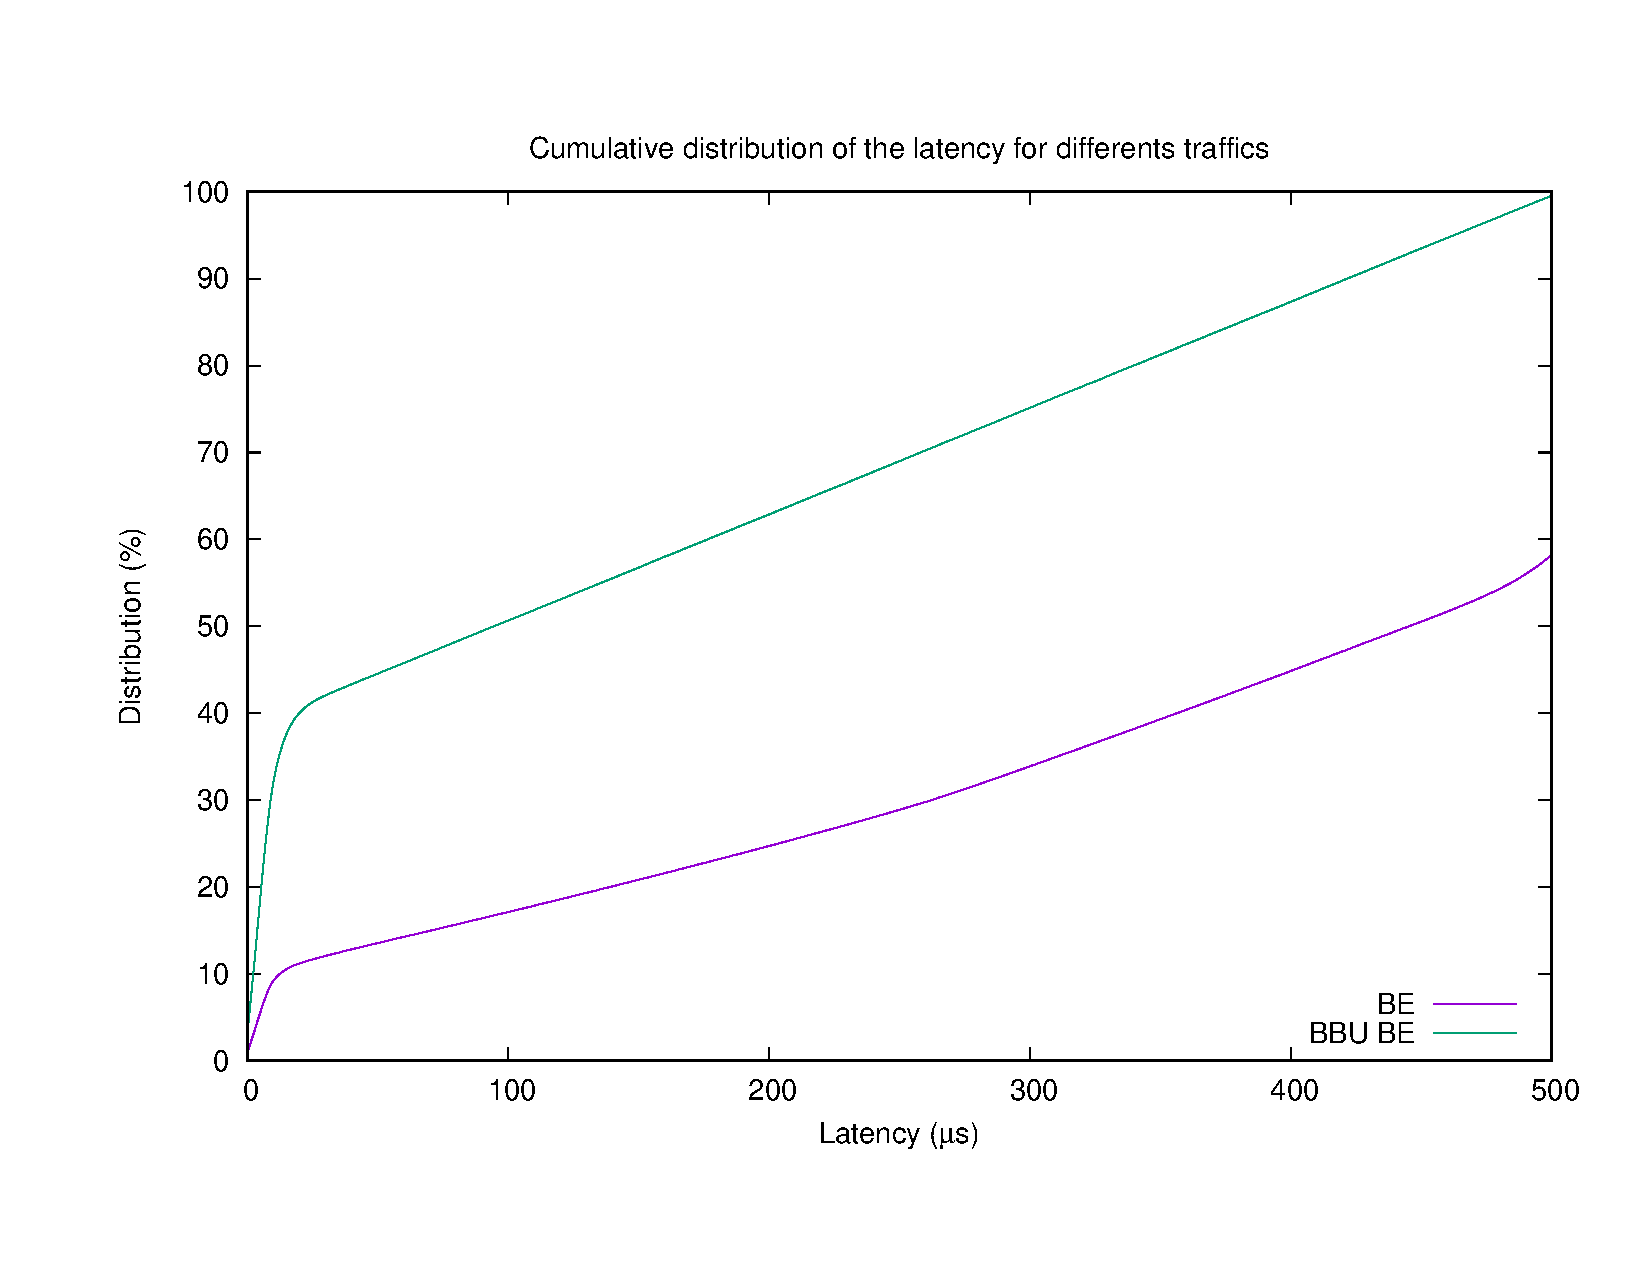
\includegraphics[scale=0.4]{res1.pdf}
     \caption{Impact of the naive reservation algorithm on the Best effort PDUs.}   \label{fig:res1}
  \end{figure}

As we can see, the BE traffic is highly penalized by this algorithm, indeed, while almost $100\%$ of the BE PDUs have a latency to less than $200 \mu$s with the full opportunistic method (see fig~\ref{fig:oport}), here, more than half of the BE PDUs are be buffered more than $200\mu s$. Those performances are explained by the structure of the algorithm. The messages are grouped together, and with our parameters, $K = 2\times n$. It creates a long sequence of slots during which there is no free containers in the ring. 

To improve the BE PDUs latnecy, we propose a {\bf splited reservation algorithm} that balances the load of the CRAN traffic over the period. Instead of giving some close BBU-offsets for all routes $i$, with $v$ the datacenter, we now uniformly distribute the different BBU-offsets in the period. Each couple BBU-RRH is still assigned to its bunch, but we split the BBU-offsets of $\frac{P}{n}$. Also, if $2 \times n < K$, the RRH are balanced over the bunches by the same way, we try to give a bunch to a RRH each $\frac{K}{2\times n}$ buches.

   \begin{figure}[!h]
\centering
      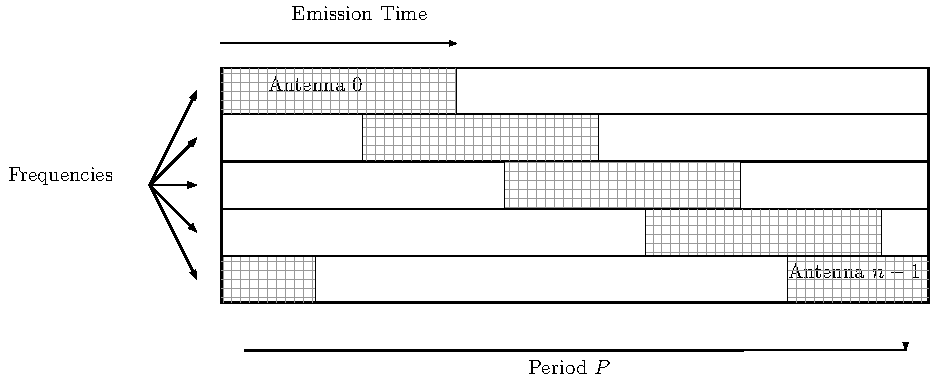
\includegraphics[scale=0.7]{freqsplited.pdf}
     \caption{Splited assignment of the bunches to the RRH.}   \label{fig:freqS}
  \end{figure}
  
  On fig~\ref{fig:res2} one can observe the performance of this algorithm on the BE PDUs latency. Once again, to have a reference point, we take the same parameters for the simulation. 

 \begin{figure}[h]
\centering
      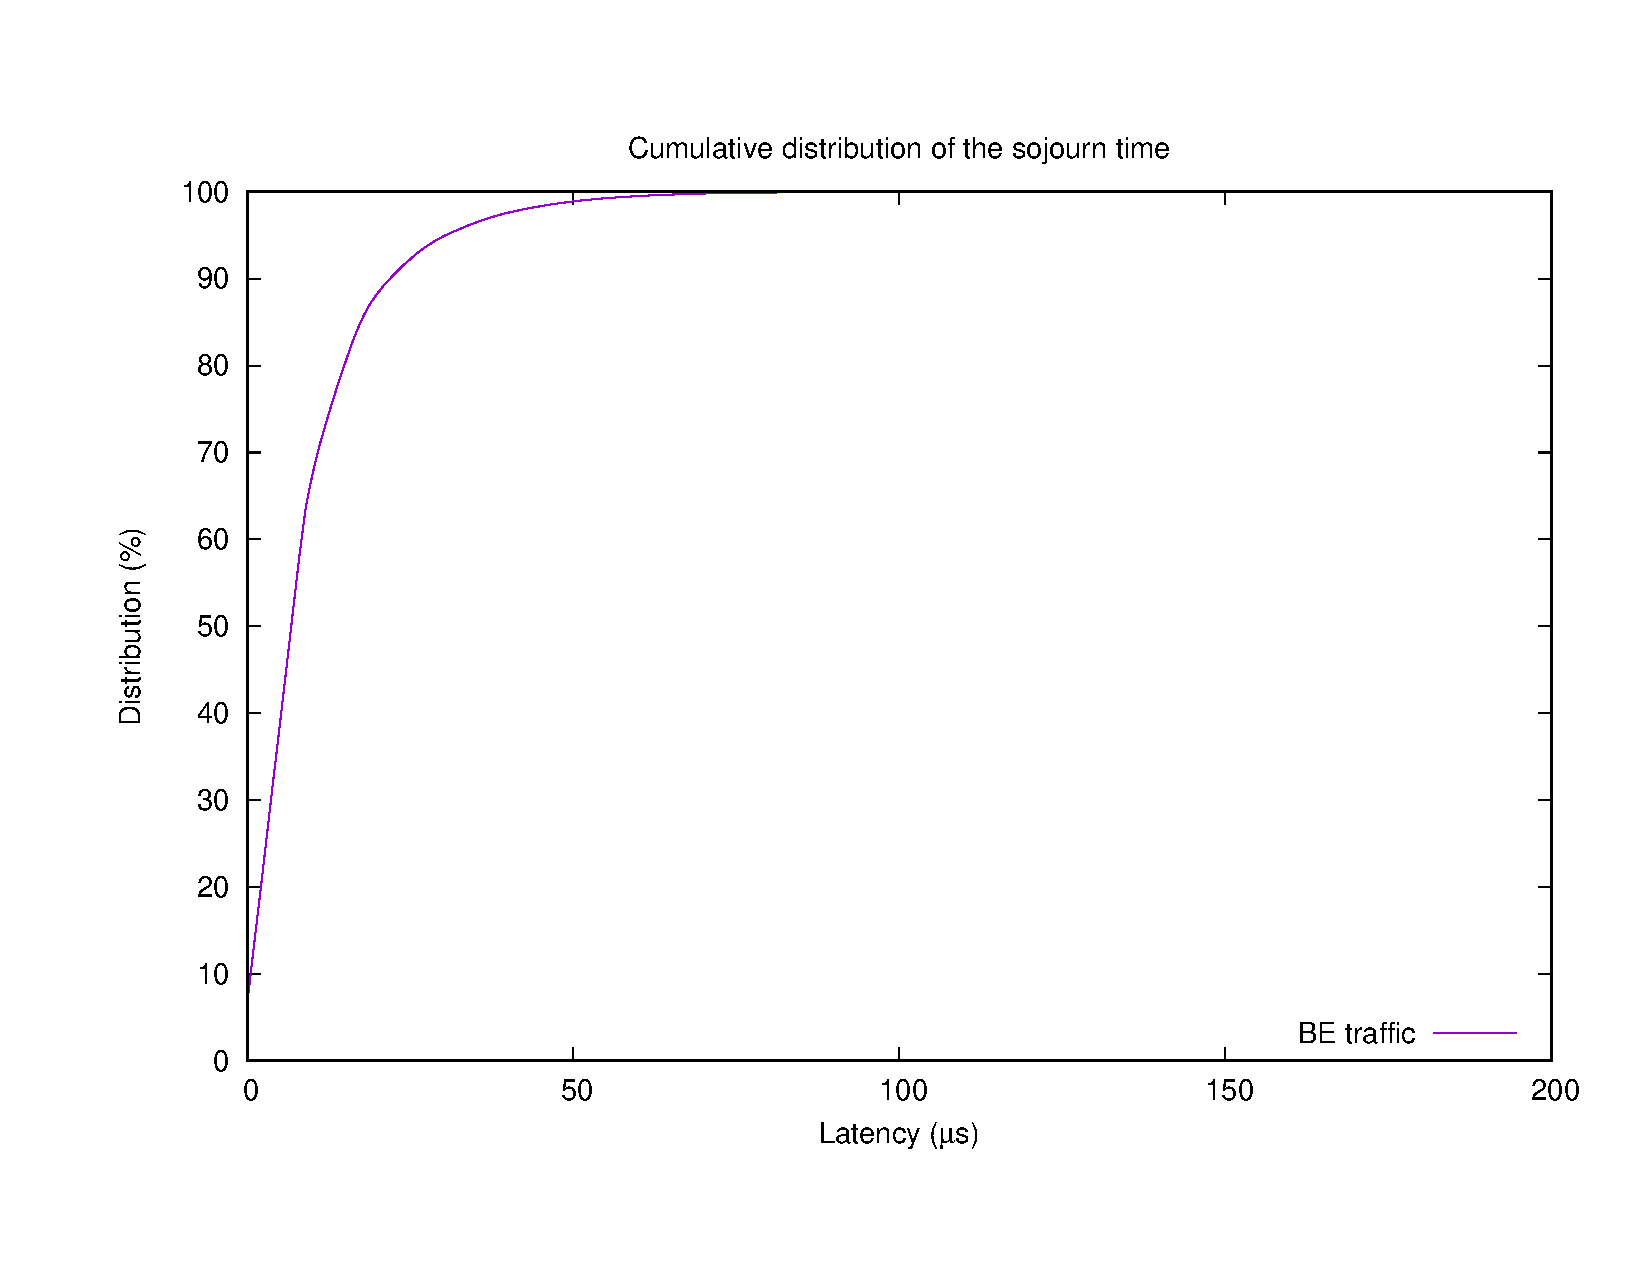
\includegraphics[scale=0.4]{res2.pdf}
     \caption{Impact of the splited reservation algorithm on the Best effort.}   \label{fig:res2}
  \end{figure}
  
  As we can see, thelatency of the BE PDUs is highly better with this this algorithm. Indeed almost $100\%$ of CRAN PDUs have a latency of less than $50\mu$s which is better than the full opportunistic method. Thus, we decreased the latency of every kind of traffic.

\subsection{With more antennas}
\label{sec:optialgo}
 In this section, we study the case $n > \frac{K}{2}$, we want to assign more than one RRH to a bunch. 
 Let us consider a particular behavior of the ring. Instinctively, we can think that if we have enough space in the period for many traffics on the same frequency that is, $ET \le \frac{P}{2}$, we can assign several couples BBU-RRH to the same bunch.

 Let us take $ET =  \frac{P}{2}$ and $n = \frac{K}{2} + 1$. We assign a bunch to each $\frac{K}{2}$ first RRH and we have only one RRH left. Then, we only look at one bunch, on which we want to add the new couple BBU-RRH. 
 
 We take a ring with two nodes $A$ and $B$. We simplify the model to only look at the behaviour of one bunch, thus, both of the nodes alternatively emits some containers every slots, during $ET$ slots in the period $P$. We assume that $A$ emits a time $1$ during $ET$ slots. This container arrives in $B$ at $\omega(A,B)$, that is  $[t(B,r_A)]_{P,K} = [\omega(A,B);\omega(A,B)+ET]$. Then, $B$ can immediately emit its containers at time $\omega(A,B)+ET$. This containers from $B$ arrives at $A$ at time $\omega(A,B)+ET + \omega(B,A) = ET + RS$, and thus, $[t(A,r_B)]_{P,K} = [ET + RS;ET + RS + ET] = [ET+RS; RS + P] = [ET + RS; RS] \mod P$. Since $[t(A,r_A)]_{P,K} = [1;ET]$, there is a collision at the interval $[1;RS]$ in the period between the two traffics from $A$ and $B$.
  \begin{figure}[h]
\centering
      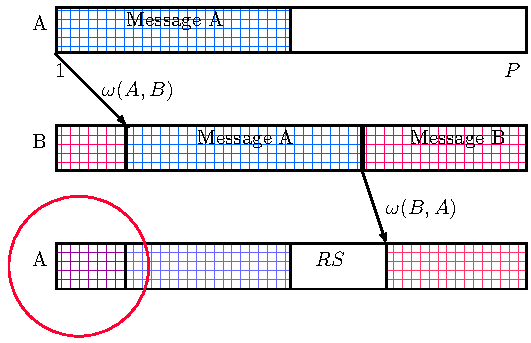
\includegraphics[scale=0.7]{rs.pdf}
     \caption{Collision between two routes on the same bunch when the period is too small.}   \label{fig:proofrs}
  \end{figure}

 
 
 As we have just noted, if several RRH share the same bunch, the period must have an additional budget in addition to the time needed to send the messages. Let us study the size of the additional budget.
 \begin{prop}
 If several RRH shares a bunch, it is possible set the offsets of the routes such that there is no collisions between the messages if $P \ge n\times ET + RS$ , with $n$ the number of RRHs.
 \end{prop}
 \begin{proof}
 We seek to show that proposition by induction.
 
 {\bf Base case:} For $n = 2$, the proof of the previous example shows us that it is possible to assign two RRH on the same bunch with $P = 2\times ET + RS$.
 
 {\bf Induction step:}  We consider that we have a bunch shared by $n$ RRH, with a period of size $P= n\times ET + RS$. We want to show that if we want to add one RRH to the bunch, we need a period of size at least $P = (n+1)\times ET + RS$. If we look at the sequence period of the bunch with $n$ RRH. We can observe that this sequence is the same in every nodes, shifted of the length of the routes between two nodes. For instance, if we take two nodes $A$ and $B$, the sequence in $A$ is the same that the sequence in $B$ shifted of $\omega(A,B)$.
 
   \begin{figure}[h]
\centering
      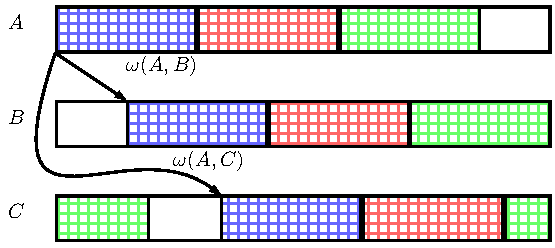
\includegraphics[scale=0.7]{period1.pdf}
     \caption{An example of sequence with n = 3.}   \label{fig:proofperiod1}
  \end{figure}
   
 Thus, if we add $ET$ slots in this bunch, the periodic emissions of all others nodes are not impacted, there is just a new interval in the sequence.
 
   \begin{figure}[h]
\centering
      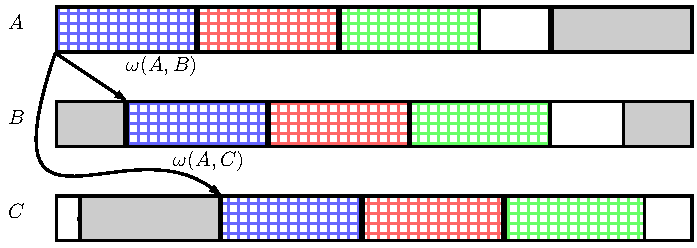
\includegraphics[scale=0.7]{period2.pdf}
     \caption{The same sequence with n = 4.}   \label{fig:proofperiod2}
  \end{figure}
  Note that a station can send some traffic from more than one RRH, the figures ~\ref{fig:proofperiod1} and \~ref{fig:proofperiod2} are just an example, but this proof stays the same.
 \end{proof}
 
Considering those results, we propose an algorithm to allow several RRH to share the same bunch, as long as $P \ge n\times ET + RS$. 
Since we need $RS$ slots on a each bunch with at least an RRH to assign another RRH to this latter, it is interesting to fill as far as possible the bunches. We then compute the number of bunches needed to carry the number of RRH $n$. Then, the algorithms tries to balance those bunches into the macro-slot, i.e. it avoids to group the used bunches together.
The used bunches have $RS$ or more free slots in the period. Thus, the algorithm subsequently balance BBU-offsets of the first RRH of each bunch, with the same idea than the splited algorithm. We call this algorithm the {\bf full repartition algorithm}. 

   \begin{figure}[h]
\centering
      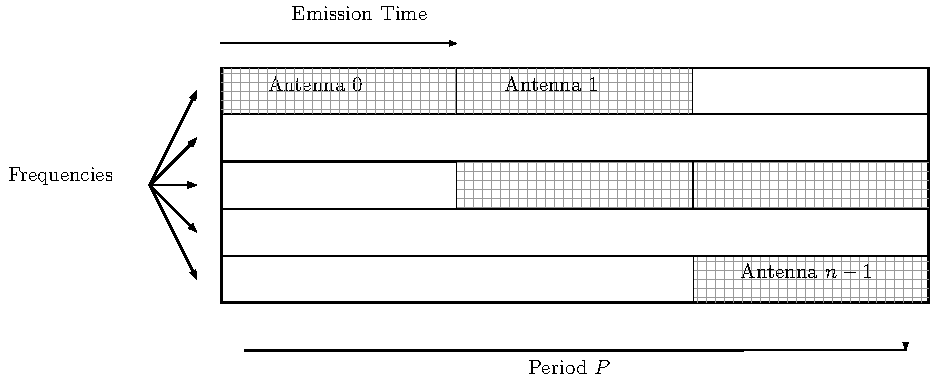
\includegraphics[scale=0.7]{optimalgo.pdf}
     \caption{Organization of the bunches with the balancing algorithm.}   \label{fig:optimalgo}
  \end{figure}
  
  We want to observe the impact of this algorithm on BE traffic. Since our previous parameters did not allow several RRH to share a bunch, we now set $ET = 200$, that correspond to a C-RAN flow of $2$Gbps. This is not out of context since the exact split (the C-RAN split is the degree of centralization of the computation units in the cloud) of the C-RAN is not fully determined yet~\cite{REF}.\todo {la ref} To keep a load similar to the load in the previous experiment, we set the number of RRH to $n=12$. The others parameters are all the one described in the sec~\ref{sec:parameters}.
  The following experiment shows us the impact of the balancing algorithm on the BE traffics. We chose to compare those results to a simulation with the same parameters but with the full opportunistic method of sec~\ref{sec:fullopport}.
  
   \begin{figure}[h]
\centering
      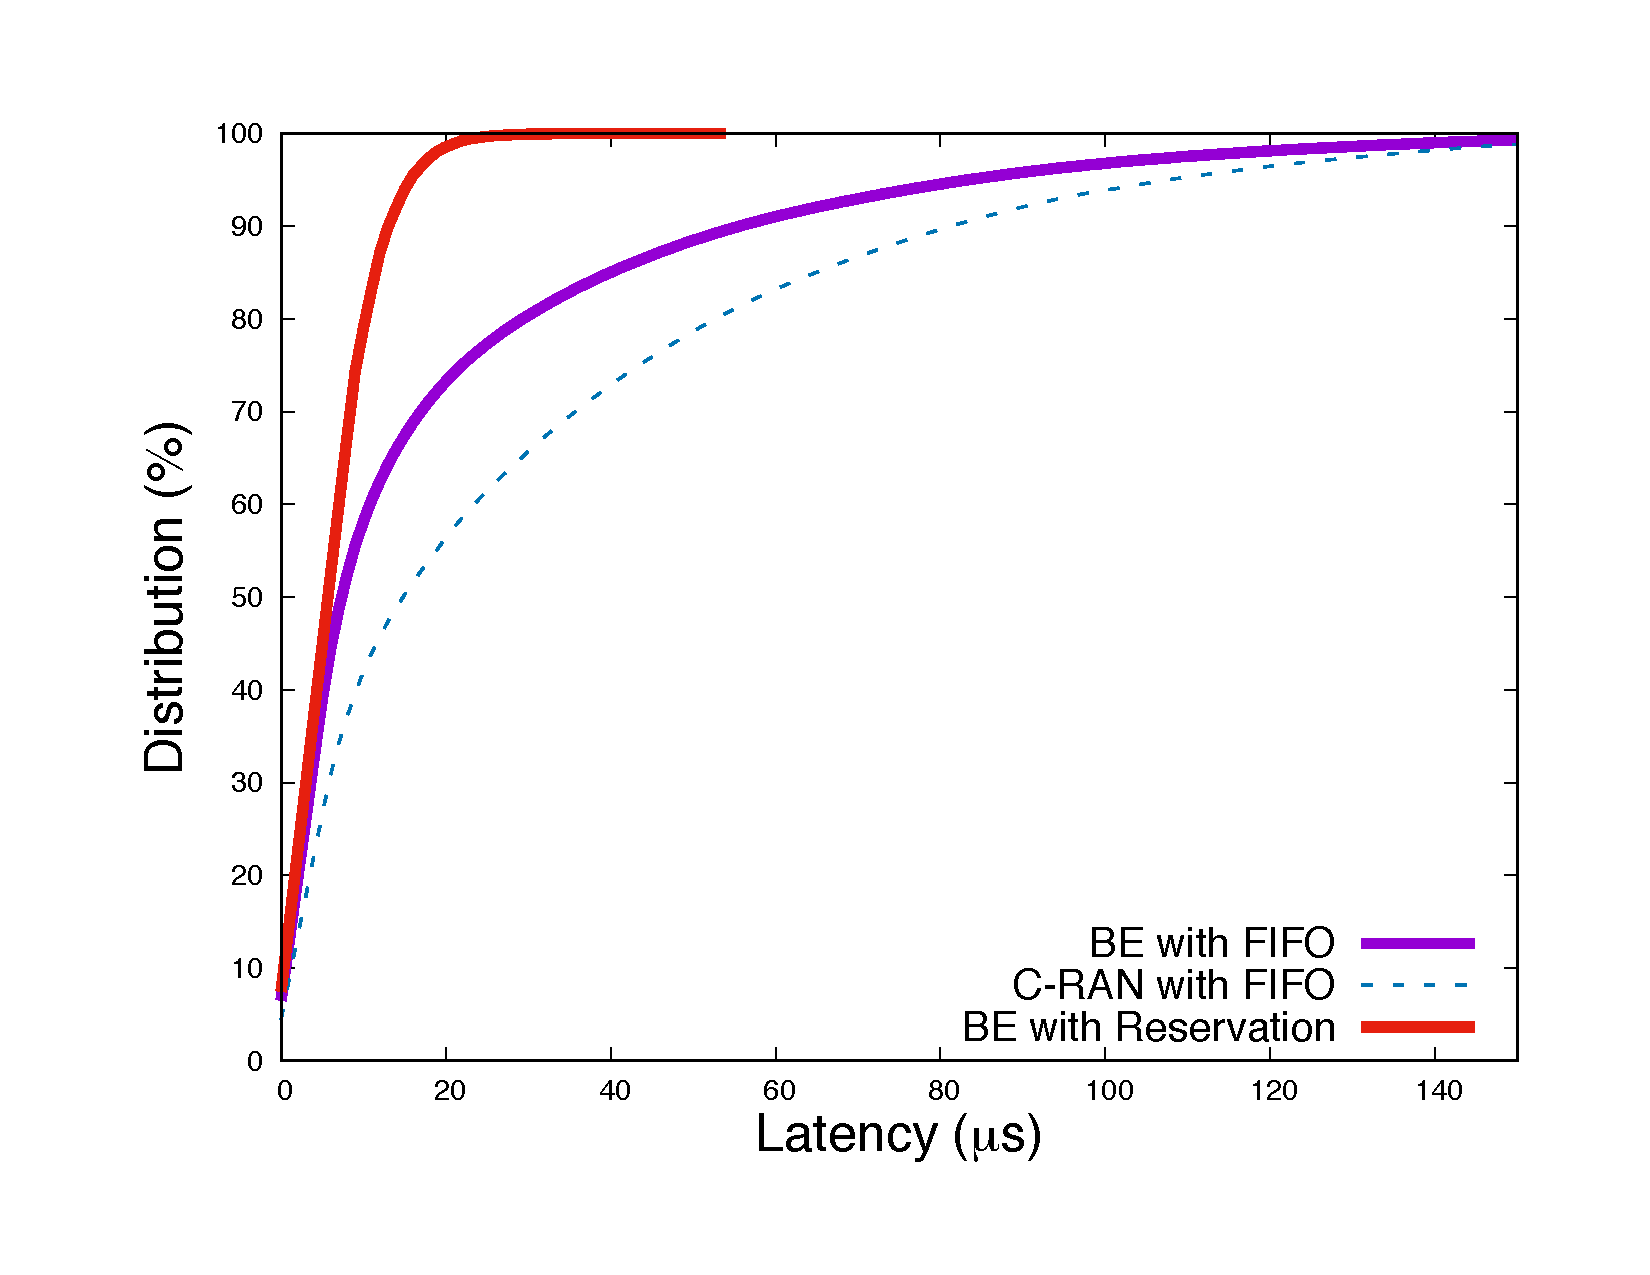
\includegraphics[scale=0.4]{optim.pdf}
     \caption{Balancing algorithm performance on the N-GREEN optical ring.}   \label{fig:optimres}
  \end{figure}
  
  As fig~\ref{fig:optimres} shows, the full repartition algorithm ensures a lower latencye to BE PDUs than the full opportunistic method, which gave the best result for the BE traffic. Indeed, since we remove the random aspect of the C-RAN PDUs generation, we balanced the load over the period an then increased the BE performances while we totally removed the C-RAN PDUs latency.
  
  \bibliographystyle{ieeetr}
\bibliography{src}

\end{document}